% 02 --- Statistical Mechanics
\section{Statistical Mechanics}

\subsection{Microstates, Macrostates, Phase Space}
\begin{frame}{Microstate vs Macrostate}
	\begin{columns}[T,onlytextwidth]
		\column{0.5\textwidth}
		\begin{pitemize}
			\item \neoncyan{Microstate}: $\Gamma = \{ \mathbf{r}^N,\mathbf{p}^N\}$ --- everything
			\item \textcolor{neonpink}{Macrostate}: $(N,V,E)$ or $(N,P,T)$ --- few numbers
			\item One macro $\leftarrow$ many micro: $\Omega$ microstates
			\item Phase space: $6N$-dim, point = microstate
		\end{pitemize}
		\column{0.5\textwidth}
		\begin{center}
			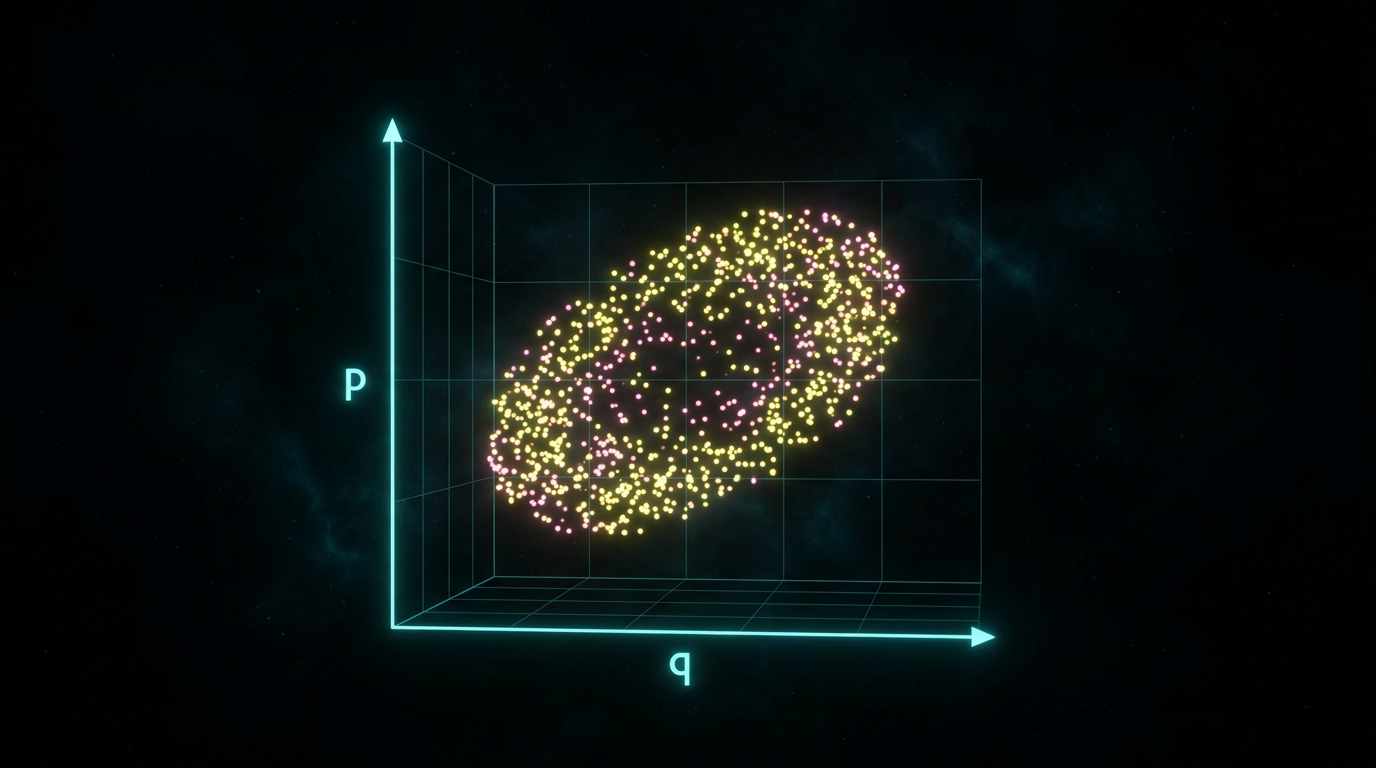
\includegraphics[width=0.9\linewidth]{assets/figures/phase_space.png}
			{\footnotesize\color{softgray} Phase space: each point = microstate}
		\end{center}
	\end{columns}
\end{frame}

\begin{frame}{Interpretation --- Micro/Macro}
	\interpret{
		\textbf{Micro} · exact positions·momenta · \textbf{macro} · thermometer numbers · \textbf{phase space} · map of all micros · \textbf{one macro} = \textbf{many micros}
	}
\end{frame}

\subsection{Energy, Entropy, Temperature}
\begin{frame}{Energy --- The Currency}
	\begin{equation*}
		E = K + U = \sum_i \frac{\mathbf{p}_i^2}{2m_i} + U(\mathbf{r}^N) \qquad \text{\color{softgray}\footnotesize micro definition}
	\end{equation*}
	\begin{columns}[T,onlytextwidth]
		\column{0.5\textwidth}
		\begin{pitemize}
			\item $U(\mathbf{r}^N)$ = PES --- see §3
			\item Conserved in NVE: $dE/dt=0$
			\item Fluctuates in NVT: $\langle (\Delta E)^2\rangle = k_BT^2 C_V$
		\end{pitemize}
		\column{0.5\textwidth}
		\begin{center}
			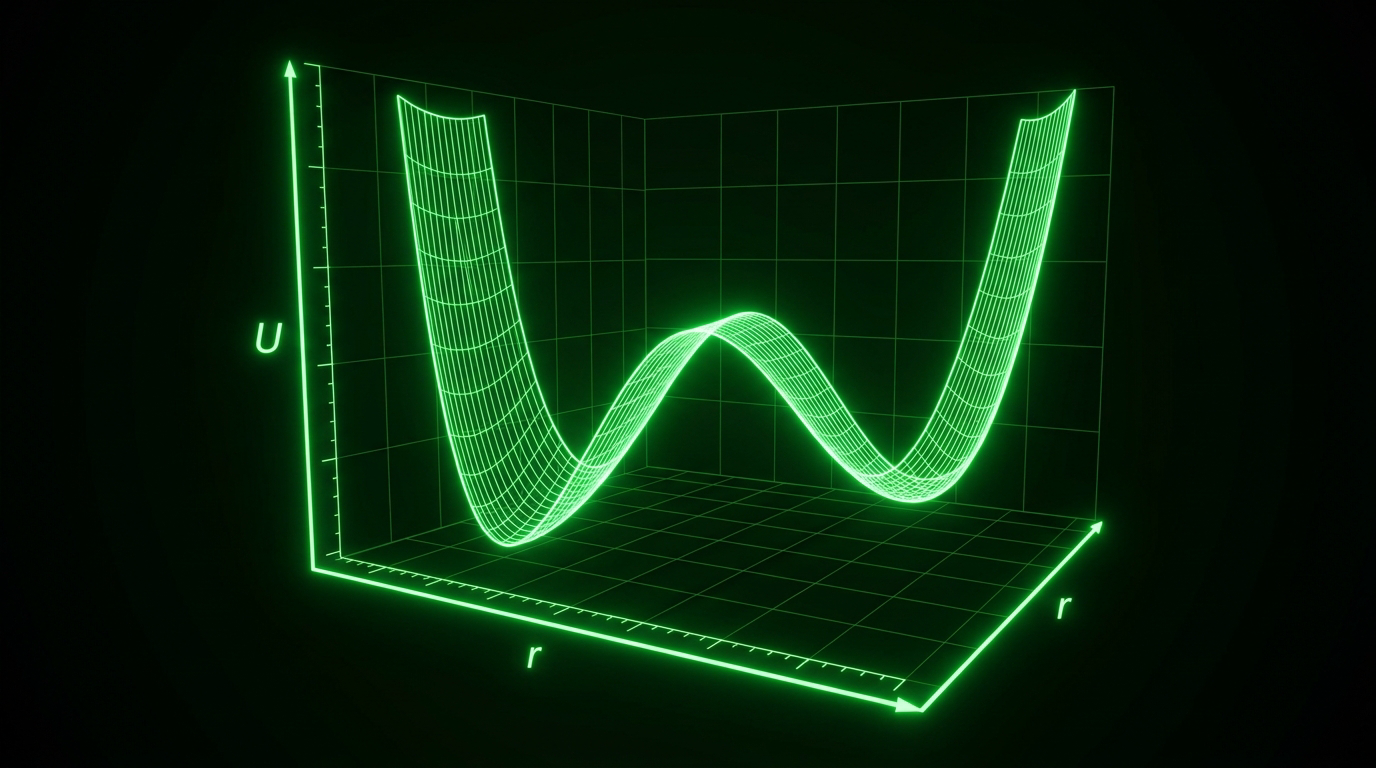
\includegraphics[width=0.9\linewidth]{assets/figures/energy_well.png}
			{\footnotesize\color{softgray} Potential energy $U(r)$: well + barrier}
		\end{center}
	\end{columns}
\end{frame}

\begin{frame}{Entropy --- Counting}
	\begin{equation*}
		S = k_B \ln \Omega \qquad\text{and}\qquad S = -k_B\sum_i p_i\ln p_i
	\end{equation*}
	\begin{columns}[T,onlytextwidth]
		\column{0.5\textwidth}
		\begin{pitemize}
			\item $\Omega$ = \# microstates for macro
			\item More ways \ensuremath{\rightarrow} more entropy \ensuremath{\rightarrow} more likely
			\item Disorder = \textbf{counting}, not mess
		\end{pitemize}
		\column{0.5\textwidth}
		\begin{center}
			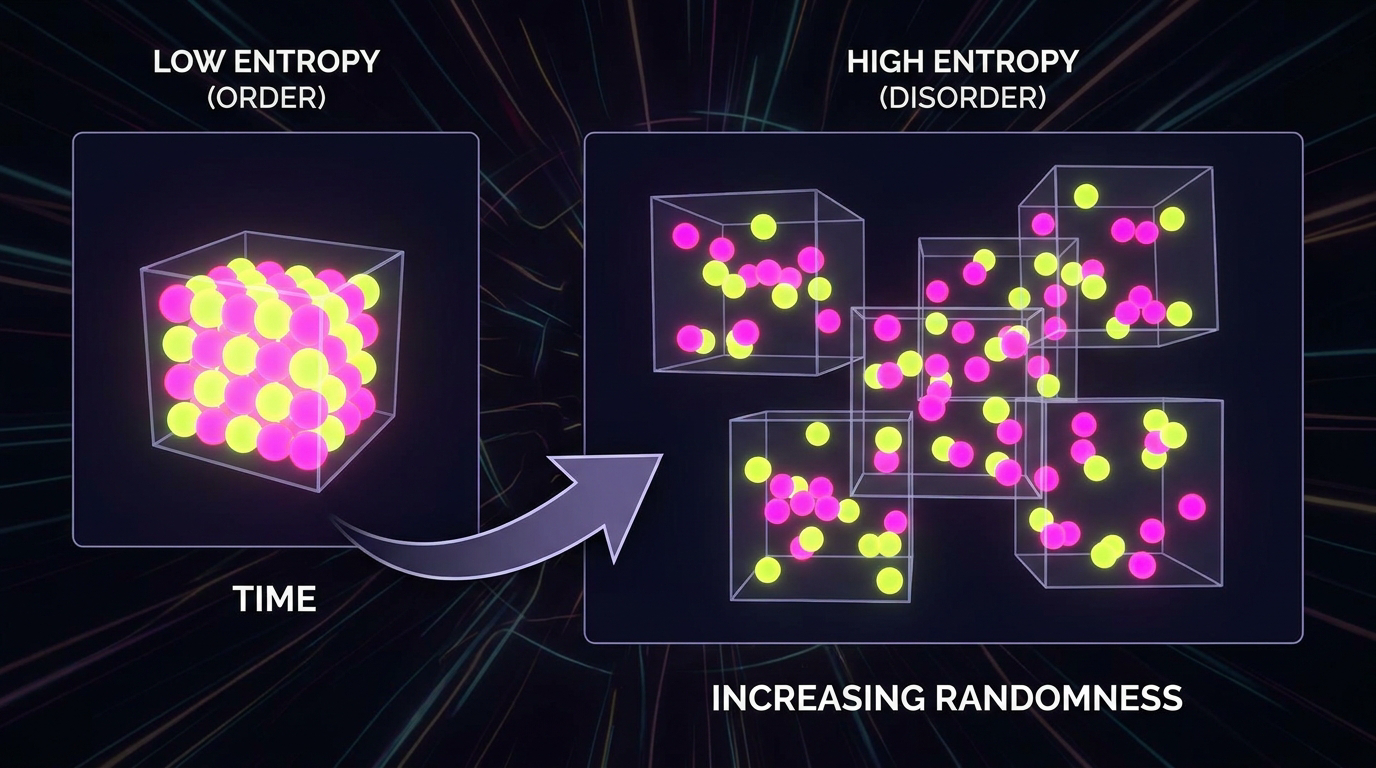
\includegraphics[width=0.9\linewidth]{assets/figures/entropy_counting.png}
			{\footnotesize\color{softgray} $\Omega=1$ (ordered) $\to$ $\Omega=10^{23}$ (disordered)}
		\end{center}
	\end{columns}
\end{frame}

\begin{frame}{Temperature --- Slope of Entropy}
	\begin{equation*}
		\frac{1}{T} = \left(\frac{\partial S}{\partial E}\right)_{N,V} \qquad
		\text{\color{softgray}hot = small slope}
	\end{equation*}
	\begin{columns}[T,onlytextwidth]
		\column{0.5\textwidth}
		\begin{pitemize}
			\item Cold: $S$ steep vs $E$
			\item Hot: $S$ flat vs $E$
			\item $T$ = \textbf{exchange rate} of $E \leftrightarrow S$
		\end{pitemize}
		\column{0.5\textwidth}
		\begin{tikzpicture}[scale=1.0]
			\draw[->,accentcyan] (0,0)--(2.8,0) node[right]{$E$};
			\draw[->,accentcyan] (0,0)--(0,2) node[above]{$S$};
			% Simple curve using coordinates instead of exp
			\draw[neongreen,thick] plot[smooth] coordinates {(0.2,0.2) (0.6,0.8) (1.0,1.2) (1.5,1.5) (2.0,1.7) (2.6,1.85)};
			\draw[dashed,neonyellow] (0.6,0) -- (0.6,0.8) -- (0,0.8);
			\node[color=neonyellow] at (0.6,-0.3) {cold $T$ low};
			\draw[dashed,neonpink] (2.0,0) -- (2.0,1.7) -- (0,1.7);
			\node[color=neonpink] at (2.0,-0.3) {hot $T$ high};
		\end{tikzpicture}
	\end{columns}
\end{frame}

\begin{frame}{Interpretation --- Energy/Entropy/Temperature}
	\interpret{
		\textbf{Energy} · conserved currency · \textbf{entropy} · count of ways · \textbf{temperature} · $dS/dE$ · \textbf{hot} = flat $S(E)$
	}
\end{frame}

\subsection{Free Energy \& Boltzmann}
\begin{frame}{Free Energy --- What Actually Matters}
	\begin{equation*}
		F = U - TS \qquad G = H - TS \qquad \min F,G \Leftrightarrow \text{stable}
	\end{equation*}
	\begin{columns}[T,onlytextwidth]
		\column{0.5\textwidth}
		\begin{pitemize}
			\item $U$ wants order, $S$ wants disorder
			\item $F$ = compromise at $T$
			\item Spontaneous $\Delta F<0$
		\end{pitemize}
		\column{0.5\textwidth}
		\memeinclude[width=0.95\linewidth]{assets/memes/boltzmann_meme.png}
	\end{columns}
\end{frame}

\begin{frame}{Boltzmann Distribution}
	\begin{equation*}
		p_i = \frac{e^{-\beta E_i}}{Z},\quad \beta=\frac1{k_BT},\quad Z=\sum_i e^{-\beta E_i}
	\end{equation*}
	\begin{columns}[T,onlytextwidth]
		\column{0.5\textwidth}
		\begin{pitemize}
			\item Low $E$ \ensuremath{\rightarrow} high $p$
			\item High $T$ \ensuremath{\rightarrow} flatter $p$
			\item $Z$ = partition function = normalization + \textbf{generator}
		\end{pitemize}
		\column{0.5\textwidth}
		\begin{center}
			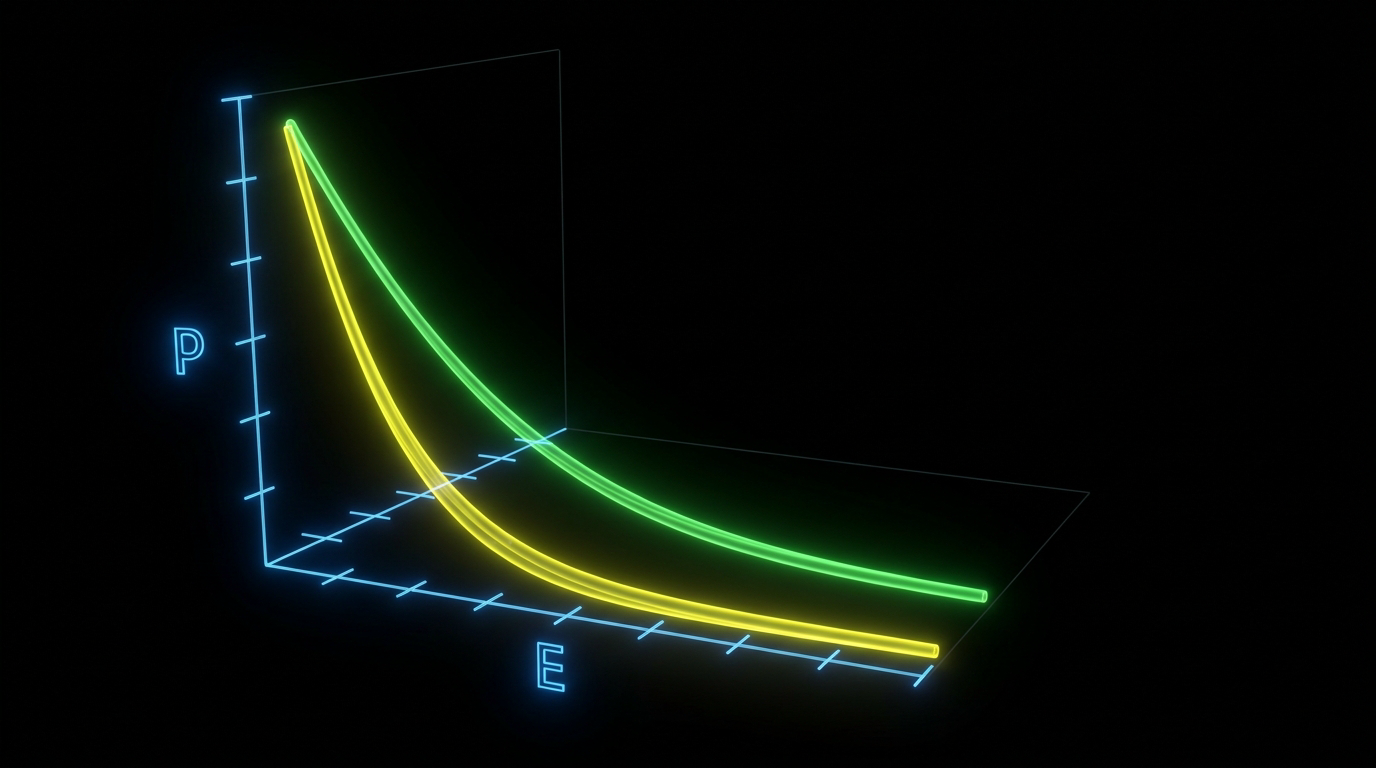
\includegraphics[width=0.9\linewidth]{assets/figures/boltzmann_dist.png}
			{\footnotesize\color{softgray} Boltzmann: cold (steep) vs hot (flat)}
		\end{center}
	\end{columns}
\end{frame}

\begin{frame}{Partition Function}
	\begin{equation*}
		Z = \sum e^{-\beta E} \;( \text{or } \int e^{-\beta H} d\Gamma ) \qquad
		F = -k_BT\ln Z
	\end{equation*}
	\begin{pitemize}
		\item $Z$ \ensuremath{\rightarrow} $F$ \ensuremath{\rightarrow} $P$, $S$, $C_V$ by derivatives
		\item Never need absolute $Z$, need \textbf{ratios} \ensuremath{\rightarrow} \textbf{sampling}
	\end{pitemize}
\end{frame}

\begin{frame}{Interpretation --- Free Energy/Boltzmann}
	\interpret{
		\textbf{free energy} · balance $U$ vs $TS$ · \textbf{Boltzmann} · low $E$ wins · \textbf{$Z$} · sum that rules them all · \textbf{cold} = picky, \textbf{hot} = tolerant
	}
\end{frame}

\subsection{Ensembles \& Ergodicity}
\begin{frame}{NVE, NVT, NPT --- Choose Your Lab}
	\begin{center}
		\begin{tikzpicture}[scale=1.0]
			\foreach \idx/\lab/\fix in {0/NVE/$E$,1/NVT/$T$,2/NPT/{$T,P$}} {
			\node[draw=accentcyan,rounded corners=2mm,fill=darkgray,minimum width=2.8cm,minimum height=1.4cm,align=center,font=\footnotesize] (b\idx) at (\idx*3.6,0) {\color{neonyellow}\bfseries \lab\\\color{fgwhite} fix \fix\\\color{softgray} micro/canonical/isobaric};
			}
			\draw[<->,thick,neongreen] (b0) -- (b1) node[midway,above,font=\footnotesize]{thermostat} ;
			\draw[<->,thick,neonpink] (b1) -- (b2) node[midway,above,font=\footnotesize]{barostat} ;
		\end{tikzpicture}
	\end{center}
	\begin{pitemize}
		\item \textbf{NVE}: isolated, $E$ conserved \ensuremath{\rightarrow} MD default
		\item \textbf{NVT}: heat bath, $T$ fixed \ensuremath{\rightarrow} biology lab
		\item \textbf{NPT}: $P$+ $T$ fixed \ensuremath{\rightarrow} real world
	\end{pitemize}
\end{frame}

\begin{frame}{Ergodicity \& Ensemble Average}
	\begin{equation*}
		\langle A\rangle = \sum_i A_i p_i \approx \frac1{T}\int_0^T A(t)\,dt \quad\text{if ergodic}
	\end{equation*}
	\begin{columns}[T,onlytextwidth]
		\column{0.5\textwidth}
		\begin{pitemize}
			\item \textbf{Ergodic}: trajectory visits all with correct weight
			\item Broken \ensuremath{\rightarrow} trapped, \textbf{rare events} matter
			\item Solution: \textbf{enhanced sampling} (§9)
		\end{pitemize}
		\column{0.5\textwidth}
		\begin{center}
			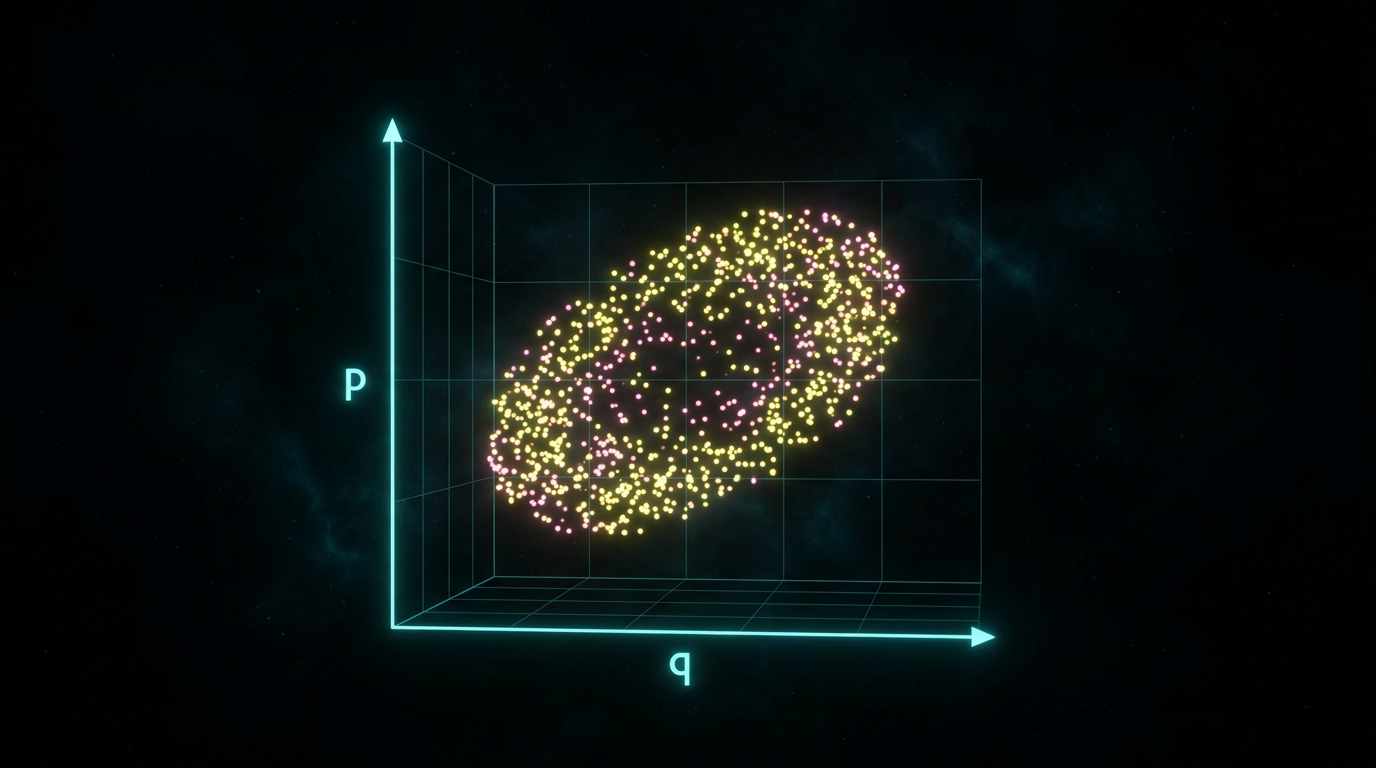
\includegraphics[width=0.9\linewidth]{assets/figures/phase_space.png}
			{\footnotesize\color{softgray} Trajectory (line) vs ensemble (shaded)}
		\end{center}
	\end{columns}
\end{frame}

\begin{frame}{Interpretation --- Ensembles}
	\interpret{
		\textbf{ensembles} · what you fix · \textbf{NVE/NVT/NPT} · lab choice · \textbf{ergodic} · time = ensemble · \textbf{broken} \ensuremath{\rightarrow} sample smarter
	}
\end{frame}
